\documentclass[a4paper]{article}
\usepackage{listings}
\usepackage{graphicx}
\lstset{basicstyle=\ttfamily}
\title{Esper4Twitter}
\author{Emanuele Dalla Longa}
\date{January 25th, 2017}
\begin{document}
\maketitle
\setlength{\parindent}{1ex}
\section{Overview}
Esper4Twitter is a software which provides an end-user interface to query the Twitter feed with the EPL language, using Esper and the official Twitter library, Hosebird Client. It has been developed for the 2016-2017 Database 2 class held by teacher Sara Comai at Politecnico di Milano.\par
It has been developed with the idea in mind that the software shouldn't be built around the query, but the other way around. So the software is highly configurable and extensible.
\section{Versions and version control}
There are two versions of the software, \lstinline$pc$ and \lstinline$rpi$. \lstinline$pc$ is the release version, which has the default configurations to run on a desktop machine. \lstinline$rpi$ is a reconfiguration of the release version which is supposed to run on a limited Raspberry Pi B machine, which sports a low-performance, single core ARM CPU.\par
The software uses Git for version control. There are two branches, one for each version. The script \lstinline$mkrelease.sh$ automatically compiles the two versions of the software and packages them in a \lstinline$.tar.gz$ archive. The release archive is meant to be uploaded to GitHub, and the other to the Raspberry Pi machine, which has been left running for 10 days. The \lstinline$rpi$ branch also contains helper scripts to process acquired data.
\section{Features}
\subsection{Output formatting}
All the queries output to a log file, which is configured in the \lstinline$log4jconfig.xml$. In the standard configuration, this is a rolling file located in \lstinline$logs/esper.log$.\par
In the \lstinline$rpi$ configuration it rotates only once a day. This is optimal since, for performance reason, this machine is meant to operate on a light \textit{user} stream instead of a data intensive \textit{sample} one. \par
The output format may be configured in the first line of the query file itself using this syntax:
\begin{lstlisting}
FORMAT "<format>"
\end{lstlisting}
where \lstinline$<format>$ is a \lstinline$printf$-like expression whose arguments are those specified in the \lstinline$select ... as$ clause as follows:
\begin{lstlisting}
MYVALUE_<NAME>
\end{lstlisting}
where \lstinline$<NAME>$ is an arbitrary value. This is easier in practice as shown in the sample queries in Section~\ref{sec:queries}.

\subsection{Queries loading}
Queries are loaded at runtime. All the files in the \lstinline$config/queries$ folder are read and parsed. If a valid format and at least a valid argument are found, a \lstinline$TweetListenerFormat$ is attached to the query, else a default \lstinline$TweetListener$ one which outputs a JSON object for each event with anonymous properties.

\subsection{Multithreading}
The software is multithreaded. Running a single while loop with no timeouts resulted in a 100\% CPU usage, so the load has been partitioned in multiple threads, thus better exploiting system resources. A 75ms timeout has been found optimal to not have any accumulation of messages in the queue while not making the CPU work in vain. The implementation of multithreading has been quite straightforward, since Esper handles multithreading natively and no resources other than the log and the message queue are shared (basically, thread input and output). The access to the message queue and to the log has been synchronized.

\subsection{Debug info}
The software has been developed with a failure-aware approach, so each action is tracked with different levels of debug. The debug level is specified in the \lstinline$log4jconfig.xml$ configuration file.

\subsection{Further possible extensions}
A handy feature to be implemented may be adding a method to the Twitter event listener which parses the hashtags and generates an event for each of them. This would enable queries directly over hashtags.

\pagebreak
\section{Acquisition work}
\subsection{Queries}
\label{sec:queries}
\paragraph{Query 1}
This query outputs the count of tweets in the last hour and the ratio of tweets with pictures over the total ones:

\begin{lstlisting}
FORMAT "%s tweets, ratio of tweets with pictures: %s"

select
 count(*) as MYVALUE_COUNT,
 (sum(
  case tweet.hasPicture() when true then 1 else 0 end 
  ) / count(*) ) as MYVALUE_RATIO 

from Tweet.win:time( 1 minute ) as tweet
\end{lstlisting} \par
The Raspberry Pi version outputs in a handy CSV format:
\begin{lstlisting}
FORMAT "%s,%s"
\end{lstlisting}

\paragraph{Query 2}
This query outputs tweets with a certain hashtag, followed by at least two tweets with pictures by the same user, which are not retweets, within 30 minutes. The rationale behind this is that this may suggest that a user has been to a certain event.

\begin{lstlisting}
FORMAT "#yolo user: %n%s%n
#yolo tweet: %n%s%n
Picture1: %n%s%n
Picture2: %n%s%n%n"

select 
 t1.user.name as MYVALUE_USER, 
 t1.text as MYVALUE_TEXT1, 
 t2[0].text as MYVALUE_TEXT2, 
 t2[1].text as MYVALUE_TEXT3

from pattern[
 every
  t1=Tweet(t1.hasHashtag("yolo")=true)
  -> [2] 
  t2=Tweet(t2.hasPicture()=true 
   and t2.user.id_str=t1.user.id_str 
   and t2.retweeted_status=null) 
   where timer:within(30 minutes) ]
      
output every 10 sec
\end{lstlisting}
\subsection{Acquired data}
In Figure \ref{fig:plot} we can see the plot of the data acquired during the 10 days of acquisition mentioned above. The red line represents the ratio of tweets with pictures over the total ones (right axis), and the black line represents the total counts of tweets (left axis). The query window duration is one hour and the granularity is 5 minutes. The origin stream is a custom \textit{user} stream which follows accounts from Italy and the US. Log files are processed with the \lstinline$datagen.sh$ script, which retrieves logs through SSH, then parses each log file and replaces the human readable timestamp with a Unix epoch, first constructing the full date using the folder name. Then they are plotted with the script \lstinline$plot.py$. The time of the day is specified in Central European Time.\par
\begin{figure}[h]
  \centerline{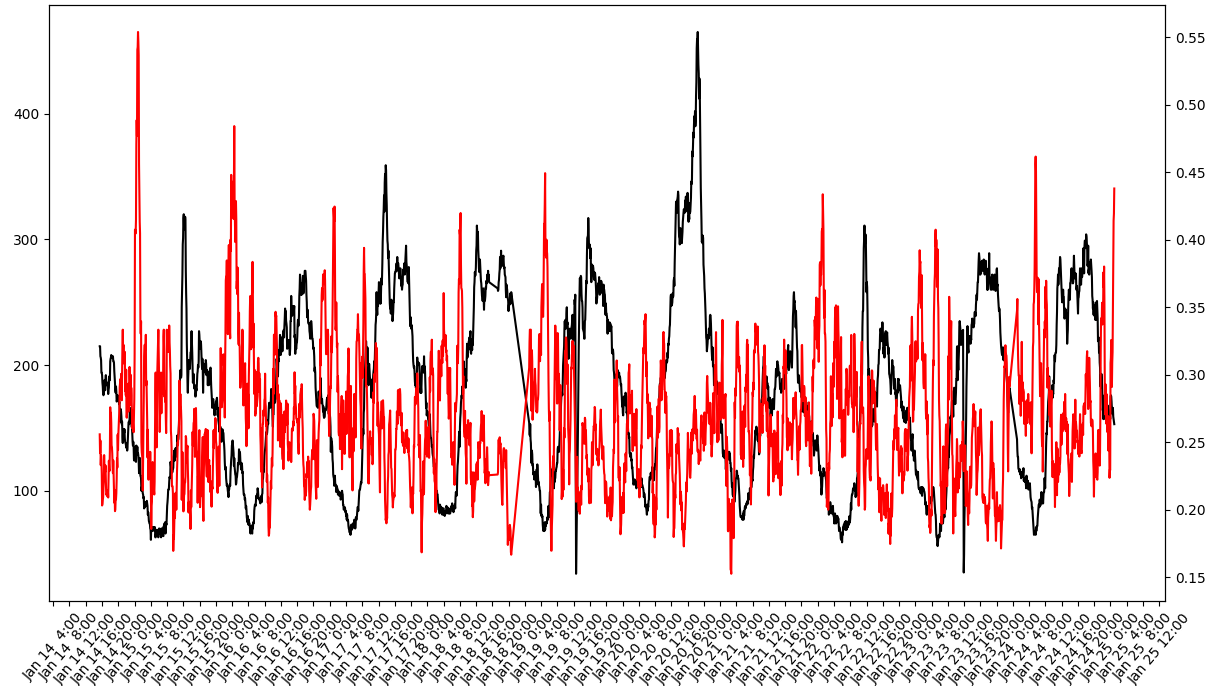
\includegraphics[width=1.5\textwidth]{figure.png}}
  \caption{Caption}
  \label{fig:plot}
\end{figure}
There is a clear spike on January 20th, during daytime. This matches with the tragic happenings in central Italy, where a hotel was hit by an avalanche. Also, there are some holes in the acquisition which match with software restarting due to version upgrading.


\end{document}